\documentclass[t]{beamer}
\usetheme[deutsch]{KIT}
\setbeamercovered{transparent}
\setbeamertemplate{navigation symbols}{}

\KITfoot{Tutoriumsmaterial von Joachim Priesner, Sebastian Ullrich und Max Wagner \hspace{2.5cm} Basierend auf den Folien von Simon Stroh und Moritz v. Looz}
\usepackage[utf8]{inputenc}
\usepackage{amsmath}
\usepackage{ifthen}
\usepackage{amssymb}
\usepackage{tikz}
\usepackage{ngerman}
\usetikzlibrary{automata}
\usenavigationsymbols


\title{Theoretische Grundlagen der Informatik}
\subtitle{Tutorium}
\author{Moritz von Looz, Simon Stroh}

\institute[ITI]{Institut für Theoretische Informatik}

\TitleImage[height=\titleimageht]{images/tmaschine.png}

\newcommand{\N}{\ensuremath{\mathbb{N}}}
\newcommand{\M}{\ensuremath{\mathcal{M}}}
\newcommand{\classP}{\ensuremath{\mathcal{P}}}
\newcommand{\classNP}{\ensuremath{\mathcal{NP}}}
\newcommand{\co}{\ensuremath{\mathsf{co\text{-}}}}
\newcommand{\pot}{\ensuremath{\mathcal{P}}}
\newcommand{\abs}[1]{\ensuremath{\left\vert #1 \right\vert}}
\newcommand{\menge}[2]{\ensuremath{\left\lbrace #1 \,\middle\vert\, #2 \right\rbrace}}
\newcommand{\ducttape}[1]{\vspace{#1}}
\newcommand{\neglit}[1]{\overline{#1\vphantom{x^a}}}
\newcommand{\recipe}{\raisebox{-.3cm}{
\includegraphics[scale=.15]{images/chefs-cap.png}}\hspace{0.2cm}}

\newcommand{\invincible}{\setbeamercovered{invisible}} %  "Yesss! I am invincible!!" (Boris Grishenko)
\newcommand{\vincible}{\setbeamercovered{transparent}}

% \@ifundefined{tikzset}{}{\tikzset{initial text=}} % Text "start" bei Startknoten unterdrücken
\tikzstyle{every node}=[thick]
\tikzstyle{every line}=[thick]

\newcommand{\tutnr}[1]{
  \subtitle{Tutorium #1}
	\begin{frame}
		\maketitle
	\end{frame}
}

\newcommand{\uebnr}[1]{
  \subtitle{Anmerkungen zum #1. Übungsblatt}
	\begin{frame}
		\maketitle
	\end{frame}
}

\begin{document}

\tutnr{6}

\subsection{Die Klasse \classNP}
\begin{frame}
\frametitle{$\mathcal{NP}$}

$\mathcal{NP}$ ist (analog zu $\mathcal{P}$) die Klasse aller Sprachen, die von einer nichtdeterministischen Turingmaschine in Polyzeit erkannt werden.

\ducttape{1cm}

\textbf{Anmerkung}: Die Frage, ob $\mathcal{P} = \mathcal{NP}$ gilt oder nicht, ist ein großes, offenes Problem.
\end{frame}

\begin{frame}
\frametitle{Grundidee: $\mathcal{NP}$-Entscheider}
Üblicherweise geht eine NTM, die ein Problem aus $\mathcal{NP}$ entscheidet, folgendermaßen vor: 
\begin{enumerate}
\item Rate sogenannten "`Zeugen"' dafür, dass $x \in L$ (nichtdeterministisch)
\item Überprüfe, ob Zeuge korrekt (in Polyzeit).
\item Falls ja akzeptiere; falls nein, lehne ab.
\end{enumerate}
Man spricht daher auch von den \emph{effizient verifizierbaren} Entscheidungsproblemen.
\end{frame}

\begin{frame}
\frametitle{$\mathcal{NP}$}

\begin{block}{Definition aus dem Skript (S.~56)}
"`Lasch"' ausgedrückt: $\Pi$ gehört zu \classNP, falls $\Pi$ folgende Eigenschaft hat:

Ist die Antwort bei Eingabe eines Beispiels $I$ von $\Pi$ "`Ja"', so kann die Korrektheit der Antwort in polynomieller Zeit überprüft werden.
\end{block}

\ducttape{1cm}

Ist diese Formulierung so korrekt?

\end{frame}

\begin{frame}
	\frametitle{Aufgabe}
	
	Sei $\mathcal{M}$ eine NTM (RV-Modell) mit Zeitkomplexitätsfunktion $T_\mathcal{M} : \N_0 \rightarrow \N$.
	
	Die Funktion $T_\mathcal{M}$ sei durch $f : \N_0 \rightarrow \N$ beschränkt und $f$ sei berechenbar.
	
	Zeige: Die von $\mathcal{M}$ akzeptierte Sprache $L(\mathcal{M})$ ist entscheidbar.
	
	\invincible \pause
	\begin{block}{Lösungsskizze}
	
	Baue TM, die $L(\mathcal{M})$ entscheidet, wie folgt: \\ Sei $x$ die Eingabe und $n := \abs{x}$.
	
	\begin{itemize}
		\item Für alle Orakelwörter bis Länge $f(n)$:
		\begin{itemize}
		\item Simuliere $\mathcal{M}$ mit aktuellem Orakelwort
		\item Falls $\mathcal{M}$ akzeptiert, akzeptiere
		\item Falls $\mathcal{M}$ mehr als $f(n)$ Schritte braucht, probiere nächstes Orakelwort
		\end{itemize}
		\item Falls $\mathcal{M}$ für kein Orakelwort akzeptiert, lehne ab.
	\end{itemize}
	\vincible
	\end{block}
\end{frame}

% NP vollständigkeit
\subsection{NP-Vollständigkeit}
\begin{frame}
\frametitle{$\mathcal{NP}$-Schwere}
\begin{block}{$\mathcal{NP}$-Schwere}
Eine Sprache $L_1$ ist $\mathcal{NP}$-schwer gdw. 
\[\forall L_2 \in \mathcal{NP} \,\, : \,\, L_2 \propto L_1\]
\end{block}
\textbf{Anmerkung}: In diesem Sinne sind die $\mathcal{NP}$-schweren Probleme schwerer oder mindestens so schwer zu lösen wie alle Probleme in $\mathcal{NP}$.
\end{frame}

% Polyreduktion ist Transitiv, daher ist NPC cool
\begin{frame}
\frametitle{Transitivität von Polyreduktionen und $\mathcal{NP}$}
Polynomielle Transformationen sind transitiv, d.h. wenn $L_1 \propto L_2$ und $L_2 \propto L_3$, dann gilt auch $L_1 \propto L_3$.\\[8pt]
Ist $L_3 \in \mathcal{NP}$, so wissen wir, dass auch $L_1$ sowie $L_2 \in \mathcal{NP}$, man spricht auch davon, $L_1$ und $L_2$ auf $L_3$ polynomiell reduziert zu haben.\\[8pt]
Gegeben eine Sprache $L_N$, von der wir wissen, dass sie $\mathcal{NP}$-schwer ist, was wäre ein möglicher Ansatz, um für eine weitere Sprache $L_X$ die $\mathcal{NP}$-Schwere zu beweisen?\\
\invincible\pause
Man zeigt $L_N \propto L_X$
\vincible
\end{frame}

\begin{frame}
\frametitle{$\mathcal{NP}$-Vollständigkeit}
Eine Sprache $L$ ist $\mathcal{NP}$-vollständig genau dann, wenn
$$L \in \mathcal{NP}$$ sowie $$L\mbox{ ist $\mathcal{NP}$-schwer}$$
Damit sind die $\mathcal{NP}$-vollständigen Probleme die "`schwersten"' Probleme aus $\mathcal{NP}$.\\
Interessant ist $\mathcal{NP}$-Vollständigkeit vor allem, da man aus Aussagen über diese Probleme viel über alle Probleme aus $\mathcal{NP}$ aussagen kann.
Ist etwa $SAT \in \mathcal{P}$, so wäre $\mathcal{P} = \mathcal{NP}$. (Warum?)
\end{frame}

\begin{frame}
\frametitle{CLIQUE}
\begin{block}{Problem}
\textbf{Gegeben:} Graph $G = (V, E)$ und ein Parameter $K \leq |V|$\\
\textbf{Frage:} Gibt es in G eine Clique der Größe mindestens $K$?
\end{block}
\begin{block}{Erinnerung}
Eine Clique ist ein vollständig verbundener Teilgraph, also eine Menge $V' \subseteq V$, so dass für alle $i,j \in V'$ mit $i\neq j$ gilt: $(i, j) \in E$.
\end{block}
\textit{Dieses Problem ist $\mathcal{NP}$-vollständig.}
\end{frame}

\begin{frame}
\frametitle{CLIQUE-Beispiel}

\begin{figure}[H]
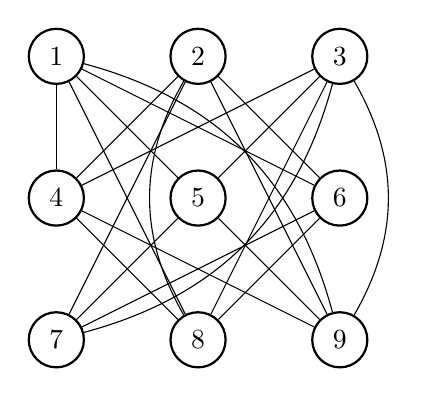
\begin{tikzpicture}[scale=1.8]
\tikzstyle{every node}=[circle, thick, minimum size = 7mm, draw]
\draw node (v1) at (0,2) {1};
\draw node (v2) at (1,2) {2};
\draw node (v3) at (2,2) {3};
\draw node (v4) at (0,1) {4};
\draw node (v5) at (1,1) {5};
\draw node (v6) at (2,1) {6};
\draw node (v7) at (0,0) {7};
\draw node (v8) at (1,0) {8};
\draw node (v9) at (2,0) {9};
\draw (v1) to (v4);
\draw (v1) to (v8);
\draw (v1) to [bend left] (v9);
\draw (v1) to (v5);
\draw (v1) to (v6);
\draw (v2) to (v4);
\draw (v2) to (v7);
\draw (v2) to [bend right] (v8);
\draw (v2) to (v9);
\draw (v2) to (v6);
\draw (v3) to (v4);
\draw (v3) to [bend left] (v7);
\draw (v3) to (v5);
\draw (v3) to (v8);
\draw (v3) to [bend left] (v9);
\draw (v4) to (v8);
\draw (v4) to (v9);
\draw (v5) to (v7);
\draw (v5) to (v9);
\draw (v6) to (v7);
\draw (v6) to (v8);
\end{tikzpicture}
\end{figure}
\begin{itemize}
\item Hat dieser Graph eine 3-CLIQUE?\pause
\item Hat dieser Graph eine 4-CLIQUE?
\end{itemize}
\end{frame}

\begin{frame}
\frametitle{$\mathcal{NP}$-Vollständigkeitsbeweis}
\begin{itemize}
 \item $CLIQUE \in \mathcal{NP}$: Übungsblatt\\
 \item $CLIQUE\mbox{ } \mathcal{NP}$ schwer: Wir zeigen $3SAT \propto CLIQUE$. (Warum?)\\\invincible\pause
 Wir müssen eine polynomielle Transformation von $3SAT$-Instanzen in $CLIQUE$-Instanzen angeben. (Warum?)\\ \vincible
\end{itemize}
\end{frame}

\begin{frame}
\frametitle{$\mathcal{NP}$-Vollständigkeitsbeweis}
Sei $C = \{c_1, \ldots, c_n\}$ eine $3SAT$-Instanz mit 
$$ c_i = x_{i1} \vee x_{i2} \vee x_{i3} \mbox{ mit } x_{ij} \in \{u_1,\ldots,u_m,\bar{u_1},\ldots,\bar{u_m}\} $$
Konstruiere eine CLIQUE-Instanz $(G = (V, E), K)$ folgendermaßen:
$$V = (v_{1,1}, v_{1,2}, v_{1,3}, v_{2,1},\ldots,v_{n,1},v_{n,2},v_{n,3})$$
$$E = {(v_{i,j},v_{k,m})| (i \neq k \wedge x_{i,j} \neq \bar{x}_{k,m} )}$$%TODO Bar sucks, \lineover or smth?
$$K = n$$
\end{frame}

\begin{frame}
\frametitle{$\mathcal{NP}$-Vollständigkeitsbeweis}
$$V = (v_{1,1}, v_{1,2}, v_{1,3}, v_{2,1},\ldots,v_{n,1},v_{n,2},v_{n,3})$$
Jeder Knoten steht also für ein Literal in der $3SAT$ Instanz. 
$$E = {(v_{i,j},v_{k,m})| (i \neq k \wedge x_{i,j} \neq \bar{x}_{k,m} )}$$%TODO Bar sucks, \lineover or smth?
Zwei Knoten sind verbunden, wenn sie gleichzeitig erfüllbar sind und nicht in der gleichen Klausel stehen. 
$$K = n$$
Wir suchen nach einer $CLIQUE$ der Größe $n$.\\
\end{frame}
\begin{frame}
\frametitle{$\mathcal{NP}$-Vollständigkeitsbeweis}
\begin{itemize}
\item Wenn eine $n$-Clique existiert:
\begin{itemize}
	\item $n$ erfüllbare Literale
	\item Alle in jeweils unterschiedlichen Formeln \\ \small{(da ja alle in einer Formel untereinander verbunden sind)}
	\item $\leadsto$ erfüllende Wahrheitsbelegung
\end{itemize}
\pause \item Wenn eine erfüllende Wahrheitsbelegung existiert:
\begin{itemize}
	\item In jeder Klausel mindestens ein Literal erfüllt
	\item Nimm aus jeder Klausel ein erfülltes Literal
	\item Bilden eine Clique nach Definition des Graphen \\ \small{"`Zwei Knoten sind verbunden, wenn sie gleichzeitig erfüllbar sind und nicht in der gleichen Klausel stehen."'}
\end{itemize}
\end{itemize}
\pause Da $CLIQUE$ $\mathcal{NP}$-schwer ist und in $\mathcal{NP}$ liegt, ist also $CLIQUE$ $\mathcal{NP}$-vollständig.
\end{frame}

\begin{frame}
\frametitle{Allgemeines zu $\classNP$-Vollständigkeitsbeweisen}
In der Regel ist es schwer zu zeigen, dass ein Problem $\mathcal{NP}$-schwer ist, aber leicht zu zeigen, dass ein Problem in $\mathcal{NP}$ liegt.\\[8pt]
Da man üblicherweise ein $\mathcal{NP}$-vollständiges Problem als Vorausetzung für die Reduktion benötigt (Ausnahme: Satz von Cook), lohnt es sich einige kennen zu lernen.
\end{frame}

\begin{frame}
	\frametitle{Bis zum nächsten Mal!}
	
	\begin{center}
		
\includegraphics[width=\textwidth]{images/221_strip.jpg}
	\end{center}
\end{frame}

\frame{
  \frametitle{Lizenzen}
  \center
  \includegraphics[width=2em]{images/by}
  \includegraphics[width=2em]{images/cc}
  \includegraphics[width=2em]{images/sa}
  \\
  {\tiny

Dieses Werk ist unter einem ``Creative Commons Namensnennung-Weitergabe unter gleichen Bedingungen 3.0 Deutschland``-Lizenzvertrag lizenziert. Um eine Kopie der Lizenz zu erhalten, gehen Sie bitte zu \href{http://creativecommons.org/licenses/by-sa/3.0/de/}{http://creativecommons.org/licenses/by-sa/3.0/de/} oder schreiben Sie an Creative Commons, 171 Second Street, Suite 300, San Francisco, California 94105, USA.\\
  \vspace{1cm}
  Davon ausgenommen sind das Titelbild, welches aus der März-April 2002 Ausgabe von American Scientist erschienen ist und ohne Erlaubnis verwendet wird, sowie das KIT Beamer Theme. Hierfür gelten die Bestimmungen der jeweiligen Urheber.
  \vspace{1cm}
  \\ 
  }
  %Habe hier die Reihenfolge etwas umgestellt, weil die Formatierung bei mir komisch aussah. 
  %Wenn es bei dir anders ist, kannst du es auch wieder zurückändern, dann haben wir unterschiedliche Kompilieroptionen
}

\end{document}